\documentclass[12pt, a4paper]{article}%Tipo de documento y tamaño de letra%

\usepackage[spanish]{babel}
\usepackage{color,graphicx}%Para poder insertar graficas%
\usepackage{graphics}
\usepackage{amsmath,amssymb}%Insertar unos símbolos matemáticos especiales%


\usepackage{silence}
\WarningFilter{latexfont}{Font shape `T1/ntxtlf/m/up' undefined}
\WarningFilter{latexfont}{Some}
\usepackage{lipsum}
\usepackage[T1]{fontenc}
\usepackage{newtxtext,euler}
\usepackage{float}
\usepackage{xcolor}
\usepackage{amsthm}
\usepackage{tikz}
\usepackage{enumerate}
\usepackage{picinpar}
% Tcolorboxes

\makeatother
\usepackage{thmtools}
\usepackage[framemethod=TikZ]{mdframed}
\mdfsetup{skipabove=1em,skipbelow=1em}

\newcommand{\sqed}{\hfill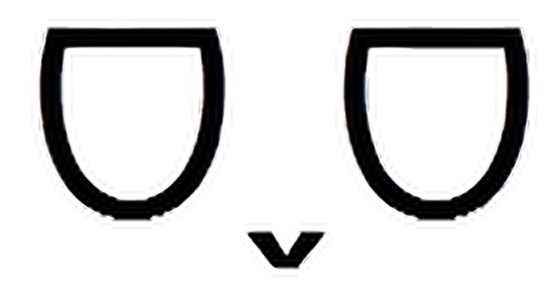
\includegraphics[height=2ex]{sancoya.png}}

\theoremstyle{definition}
\declaretheoremstyle[
    headfont=\bfseries\sffamily\color{black!70!black}, bodyfont=\normalfont,
    mdframed={
        linewidth=0.7pt,
        rightline=true, topline=true, bottomline=true,
        linecolor=black, backgroundcolor=black!2!white,
    }
]{thmbox}

\declaretheoremstyle[
    headfont=\bfseries\sffamily\color{black!70!black}, bodyfont=\normalfont,
    numbered=no,
    mdframed={
        linewidth=0pt,
        rightline=false, topline=false, bottomline=false,
        linecolor=black, backgroundcolor=black!1.5!white,
    },
    qed=\qedsymbol
]{thmproofbox}

\declaretheoremstyle[
    headfont=\bfseries\sffamily\color{black!70!black}, bodyfont=\normalfont,
    numbered=no,
    mdframed={
        linewidth=0pt,
        rightline=false, topline=false, bottomline=false,
        linecolor=black, backgroundcolor=black!1.5!white,
    },
    qed=\sqed
]{sancoya}


\declaretheorem[style=thmbox, name=Definición]{definition}
\declaretheorem[style=thmbox, numbered=no, name=Ejemplo]{eg}
\declaretheorem[style=sancoya, numbered=no, name=Demostración]{sproof}
\declaretheorem[style=thmbox, name=Proposición]{prop}
\declaretheorem[style=thmbox, name=Teorema, numbered=no]{theorem}
\declaretheorem[style=thmbox, name=Lema]{lemma}
\declaretheorem[style=thmbox, numbered=no, name=Corolario]{corollary}


\declaretheorem[style=thmproofbox, name=Demostración]{replacementproof}
\renewenvironment{proof}[1][\proofname]{\vspace{-10pt}\begin{replacementproof}}{\end{replacementproof}}


\declaretheorem[style=thmbox, numbered=no, name=Nota]{note}
\declaretheorem[style=thmbox, numbered=no, ]{temp}




\usepackage{geometry}
 \geometry{
 a4paper,
 total={170mm,245mm},
 left=25mm,
 top=30mm,
 }

\begin{document}

\setlength{\parindent}{0cm}
\hoffset-0.46cm
\voffset-1.46cm

\begin{window}[0,l,{
\includegraphics[scale=0.31]{logo.eps}},]
\large\scshape  \hspace{0.4cm}\textsf{Universidad Nacional de Colombia} \\
\textcolor{white}{\tiny.}  \large \hspace{1.5cm} \textsf{Facultad de Ciencias} \\
\textcolor{white}{\tiny.}   \normalsize\hspace{0.7cm}\textsf{Teoria de Codificación}\\
 

\end{window}

\vspace{0.2cm}
\small
\textsf{Edgar Santiago Ochoa Quiroga\\
María Alejandra  Rodríguez  Ríos} 
\normalsize
\dotfill
\vspace{0.7cm}

%Ella a mí siempre me trasnocha, yo la pienso a toda hora, pasa por su casa bien sola, deseo que ella sea mi esposa, y anoche yo me presenté en su casa, le dije to' lo que ella a mí me gustaba, ella me dijo "ay papi, qué bonito, échate pa' acá un poquito". Se me fue acercando poco a poquito, con la primera cita ella me dio un besito, me dijo que fuéramos noviecitos y le quité el shorcito. Y la encendí a mondá en la sala de su casa y terminamos en la terraza, yo le pegué su mondaquera en la cama, esa muchacha como gritaba.%





 \end{document}